% Drawing 83/01-4 -- folder 83, batch 01, archive page 15 (PDF page 16).
% Transcription: à gauche de l'énoncé, l'étoile pentagonale d'un sommet $u_0$, avec une arête épaissie vers $u_1$.
% Kind: star of a vertex (pentagon). Method 2 (schematic redraw from the facsimile). Status: ok.
% Notes: Pentagonal star of u_0: five spokes and the pentagon. Two spokes are thickened, towards the top right vertex and towards the right vertex labelled u_1 (the transcription names one thickened edge, towards u_1).
% Coordinates: 1 unit = 1 mm = 1/100 of the crop width (bbox in page fractions: [0.15, 0.24, 0.33, 0.34]).
% Redrawn by Claude (claude-opus-5-5), issue #73, 2026-11-07; not checked by a human; not compiled (no TeX in the session).
% Rights: reproduces part of the work -- behind RENDER_TRANSCRIPTS, never published by itself.
\documentclass[tikz,border=3pt]{standalone}
\usepackage{amsmath,amssymb}
\usetikzlibrary{patterns,arrows.meta}
\tikzset{pencil/.style={black!45}, struck/.style={black!35}, mark/.style={circle,draw,inner sep=1.3pt}, pt/.style={circle,fill,inner sep=0.9pt}, opt/.style={circle,draw,fill=white,inner sep=1.1pt}}
\begin{document}
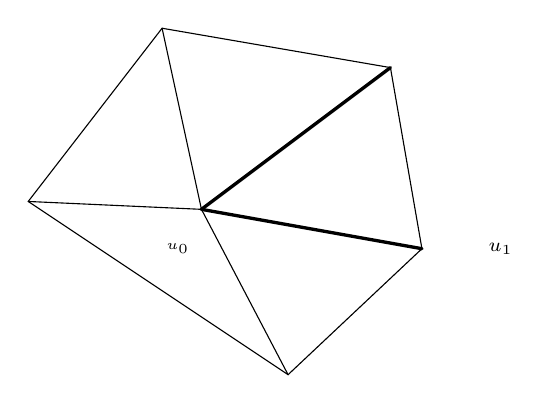
\begin{tikzpicture}[x=1mm,y=1mm,line cap=round,line join=round,font=\scriptsize]
\draw (40,-22) -- (69,-27);
\draw (69,-27) -- (73,-50);
\draw (73,-50) -- (56,-66);
\draw (56,-66) -- (23,-44);
\draw (23,-44) -- (40,-22);
\draw (45,-45) -- (40,-22);
\draw (45,-45) -- (56,-66);
\draw (45,-45) -- (23,-44);
\draw[very thick] (45,-45) -- (69,-27);
\draw[very thick] (45,-45) -- (73,-50);
\node[inner sep=1pt] at (42,-50) {\tiny $u_0$};
\node[inner sep=1pt] at (83,-50) {\scriptsize $u_1$};
\end{tikzpicture}
\end{document}
